\documentclass{article}

% ======================================================================
% Edit-response geometry of a frozen genomic foundation model -- preprint
% (NeurIPS 2025 style, preprint mode)
% Build:  make   (tectonic, two passes)
% ======================================================================
\usepackage[preprint,nonatbib]{neurips}

\usepackage[utf8]{inputenc}
\usepackage[T1]{fontenc}
\usepackage{microtype}
\usepackage{amsmath,amssymb,amsfonts}
\usepackage{mathtools}
\usepackage{booktabs}
\usepackage{multirow}
\usepackage{array}
\usepackage{graphicx}
\usepackage{float}
\usepackage{xcolor}
\usepackage{tikz}
\usepackage{pgfplots}
\pgfplotsset{compat=1.18}
\usetikzlibrary{arrows.meta,positioning,fit,backgrounds,calc,shapes.symbols,patterns}
\usepackage[numbers,sort&compress]{natbib}
\usepackage{url}
\usepackage[colorlinks=true,allcolors=blue!55!black,breaklinks=true]{hyperref}
\usepackage{cleveref}
\usepackage{enumitem}
\usepackage{xspace}

\newcommand{\up}{$\uparrow$\xspace}
\newcommand{\dn}{$\downarrow$\xspace}

% --- canonical notation (notation contract) ---
\newcommand{\Real}{\mathbb{R}}
\newcommand{\enc}{\mathrm{enc}}
\newcommand{\sref}{s_{\mathrm{ref}}}
\newcommand{\salt}{s_{\mathrm{alt}}}
\newcommand{\D}{\Delta}
\newcommand{\Dhat}{\hat\Delta}
\newcommand{\gpred}{g}
\newcommand{\wref}{w_{\mathrm{ref}}}
\newcommand{\walt}{w_{\mathrm{alt}}}
\newcommand{\carbon}{Carbon-500M\xspace}
\newcommand{\method}{GenoLeWM\xspace}
\newcommand{\eg}{e.g.,\xspace}
\newcommand{\ie}{i.e.,\xspace}

% ======================================================================
% figures.tex  --  all figures for the GenoLeWM paper.
% Self-contained: requires tikz, pgfplots, xcolor (loaded in main preamble).
% Color + style definitions are guarded so this file also compiles standalone.
% ======================================================================
\providecommand{\genocolor}{}\definecolor{genocolor}{HTML}{2F6F9F}
\providecommand{\carboncolor}{}\definecolor{carboncolor}{HTML}{C24A3B}
\providecommand{\baselinecolor}{}\definecolor{baselinecolor}{HTML}{8A8A8A}
\definecolor{statefill}{HTML}{EAF1F7}
\definecolor{actfill}{HTML}{FBE9E6}

% ----------------------------------------------------------------------
% Figure 1: system architecture / latent-edit pipeline
% ----------------------------------------------------------------------
\newcommand{\figArchitecture}{%
\begin{figure}[t]
  \centering
  \resizebox{\linewidth}{!}{%
  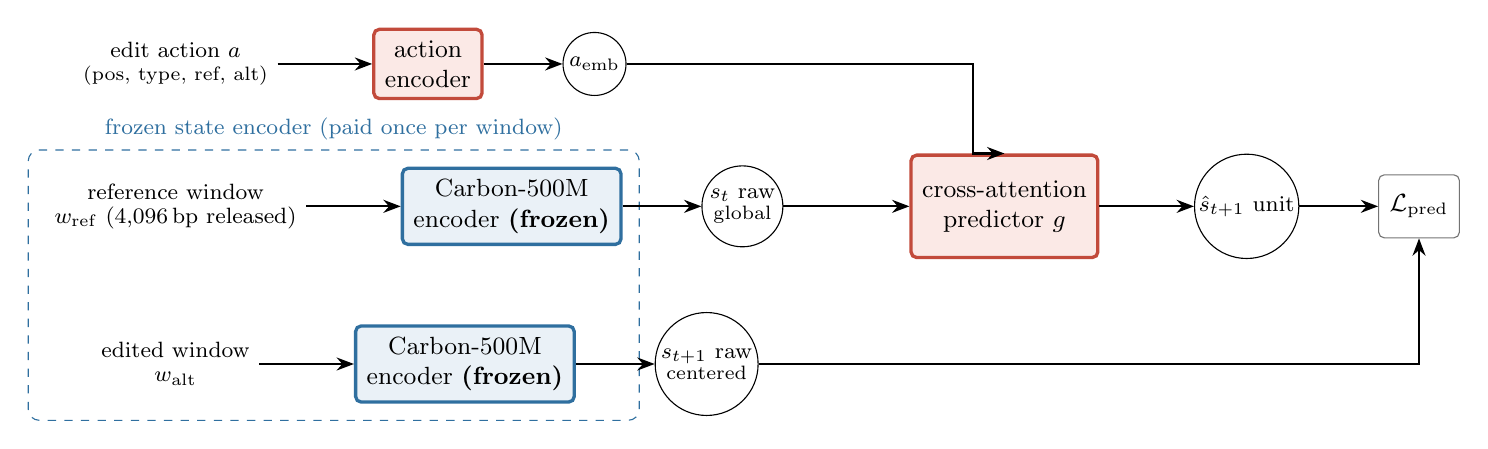
\begin{tikzpicture}[
    font=\small,
    box/.style={draw,rounded corners=2pt,minimum height=8mm,inner sep=4pt,align=center},
    frozen/.style={box,draw=genocolor,fill=statefill,very thick},
    train/.style={box,draw=carboncolor,fill=actfill,very thick},
    io/.style={align=center,font=\footnotesize},
    lat/.style={circle,draw,minimum size=8mm,inner sep=1pt,font=\footnotesize,align=center},
    arr/.style={-{Stealth[length=2.2mm]},thick},
  ]
    \node[io] (edit) {edit action $a$\\[-1pt]\scriptsize(pos, type, ref, alt)};
    \node[io,below=10mm of edit] (wref) {reference window\\[-1pt]$w_{\mathrm{ref}}$ ($4{,}096$\,bp released)};
    \node[io,below=12mm of wref] (walt) {edited window\\[-1pt]$w_{\mathrm{alt}}$};

    \node[train,right=12mm of edit] (aenc) {action\\encoder};
    \node[frozen,right=12mm of wref] (enc1) {Carbon-500M\\encoder \textbf{(frozen)}};
    \node[frozen,right=12mm of walt] (enc2) {Carbon-500M\\encoder \textbf{(frozen)}};

    \node[lat,right=10mm of aenc] (aemb) {$a_{\mathrm{emb}}$};
    \node[lat,right=10mm of enc1] (st) {$s_t$ raw\\[-2pt]\scriptsize global};
    \node[lat,right=10mm of enc2] (stp1) {$s_{t+1}$ raw\\[-2pt]\scriptsize centered};

    \node[train,right=16mm of st,minimum height=13mm] (pred) {cross-attention\\predictor $g$};
    \node[lat,right=12mm of pred] (shat) {$\hat s_{t+1}$ unit};
    \node[box,draw=black!55,right=10mm of shat] (loss) {$\mathcal{L}_{\mathrm{pred}}$};
    \draw[arr] (edit) -- (aenc);
    \draw[arr] (wref) -- (enc1);
    \draw[arr] (walt) -- (enc2);
    \draw[arr] (aenc) -- (aemb);
    \draw[arr] (enc1) -- (st);
    \draw[arr] (enc2) -- (stp1);
    \draw[arr] (aemb) -| ([xshift=-4mm]pred.north) -- (pred.north);
    \draw[arr] (st) -- (pred);
    \draw[arr] (pred) -- (shat);
    \draw[arr] (shat) -- (loss);
    \draw[arr] (stp1) -| (loss.south);
    \begin{scope}[on background layer]
      \node[fit=(enc1)(enc2)(wref)(walt),draw=genocolor,dashed,rounded corners,inner sep=6pt,
        label={[genocolor,font=\footnotesize]above:frozen state encoder (paid once per window)}] {};
    \end{scope}
  \end{tikzpicture}}
  \caption{\textbf{Released v0.2.1-r1 computation, exposing the state-contract violation.}
  A frozen Carbon-500M DNA encoder maps a reference window $w_{\mathrm{ref}}$ to a state
  $s_t\in\mathbb{R}^{1024}$; a small trainable action encoder maps an explicit edit
  $a=(\text{pos},\text{type},\text{ref},\text{alt})$ to $a_{\mathrm{emb}}$; and a cross-attention
  predictor $g$ returns $\hat s_{t+1}=g(s_t,a_{\mathrm{emb}})$. Although \texttt{normalize: true} was
  configured, released source and target encoder states were raw (rollout mean norms $29$--$34$), while
  the predictor output was unit norm. Training sources used global pooling while targets used edit-centered
  pooling; every nominal edit center also omitted the leading \texttt{<dna>} token and was shifted one hidden token left.
  Rollout changed the source coordinate again. The frozen target-only KL had no gradient and no LoRA was present.
  The diagram documents implementation flow, not validated world-model capability.}
  \label{fig:architecture}
\end{figure}}

% ----------------------------------------------------------------------
% Figure 2: VEP results vs Carbon zero-shot
% ----------------------------------------------------------------------
\newcommand{\figVEP}{%
\begin{figure}[t]
  \centering
  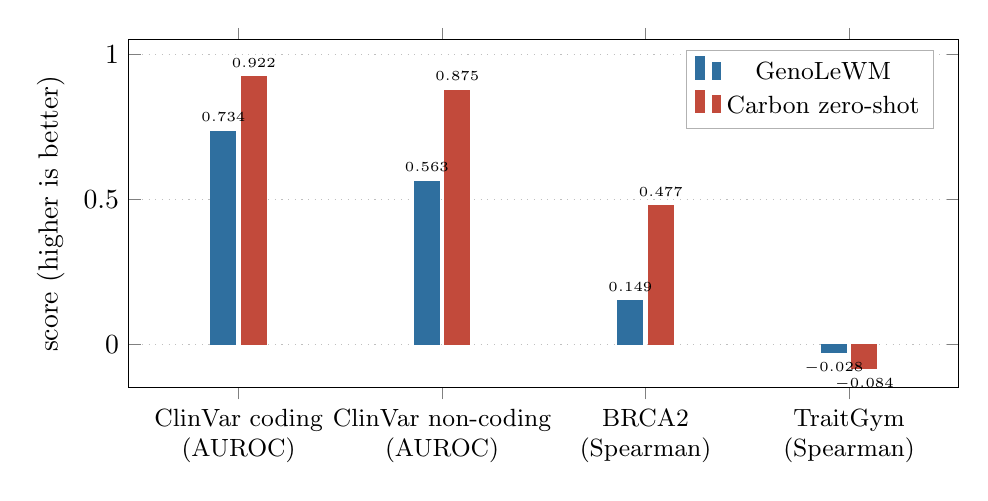
\begin{tikzpicture}
  \begin{axis}[
    width=\linewidth, height=6cm, ybar, bar width=9pt,
    ymin=-0.15, ymax=1.05,
    ylabel={score (higher is better)},
    symbolic x coords={ClinVar coding\\(AUROC),ClinVar non-coding\\(AUROC),BRCA2\\(Spearman),TraitGym\\(Spearman)},
    xtick=data, xticklabel style={align=center,font=\small},
    legend pos=north east, legend style={font=\small,draw=black!30},
    enlarge x limits=0.18, ymajorgrids, grid style=dotted,
    nodes near coords, every node near coord/.append style={font=\tiny,/pgf/number format/.cd,fixed,precision=3},
  ]
  \addplot[fill=genocolor,draw=genocolor] coordinates {
    ({ClinVar coding\\(AUROC)},0.734375)
    ({ClinVar non-coding\\(AUROC)},0.5625)
    ({BRCA2\\(Spearman)},0.149194)
    ({TraitGym\\(Spearman)},-0.0279645)};
  \addplot[fill=carboncolor,draw=carboncolor] coordinates {
    ({ClinVar coding\\(AUROC)},0.921875)
    ({ClinVar non-coding\\(AUROC)},0.875)
    ({BRCA2\\(Spearman)},0.476907)
    ({TraitGym\\(Spearman)},-0.0838935)};
  \legend{GenoLeWM, Carbon zero-shot}
  \end{axis}
  \end{tikzpicture}
  \caption{\textbf{Historical v0.2.1 VEP rows; withdrawn as a method comparison.} Carbon values are
  recovered as GenoLeWM~$-$~$\Delta$. The GenoLeWM ranking score came from an $L_2$ residual between
  unit-norm predictions and raw target states, so bar differences do not establish better or worse
  performance for the intended normalized-state method. The small slices add a separate power
  limitation; see \S\ref{sec:limitations}.}
  \label{fig:vep}
\end{figure}}

% ----------------------------------------------------------------------
% Figure 3: rollout fidelity vs source-state baseline (the baseline trap)
% ----------------------------------------------------------------------
\newcommand{\figRollout}{%
\begin{figure}[t]
  \centering
  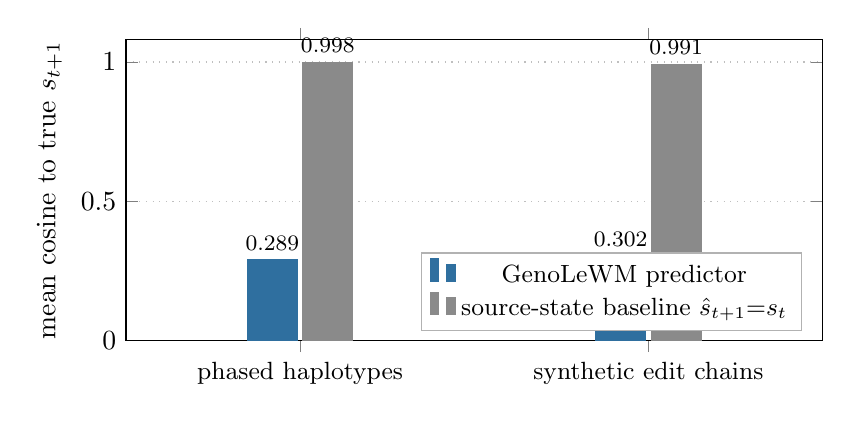
\begin{tikzpicture}
  \begin{axis}[
    width=0.86\linewidth, height=5.4cm, ybar, bar width=18pt,
    ymin=0, ymax=1.08,
    ylabel={mean cosine to true $s_{t+1}$},
    symbolic x coords={phased haplotypes,synthetic edit chains},
    xtick=data, xticklabel style={font=\small},
    legend pos=south east, legend style={font=\small,draw=black!30},
    enlarge x limits=0.5, ymajorgrids, grid style=dotted,
    nodes near coords, every node near coord/.append style={font=\footnotesize,/pgf/number format/.cd,fixed,precision=3},
  ]
  \addplot[fill=genocolor,draw=genocolor] coordinates {(phased haplotypes,0.288861) (synthetic edit chains,0.301608)};
  \addplot[fill=baselinecolor,draw=baselinecolor] coordinates {(phased haplotypes,0.997831) (synthetic edit chains,0.991239)};
  \legend{GenoLeWM predictor, source-state baseline $\hat s_{t+1}{=}s_t$}
  \end{axis}
  \end{tikzpicture}
  \caption{\textbf{Historical rollout cosine; mechanism withdrawn.} Prediction-to-target cosine is
  $\approx0.29$--$0.30$ and raw-source-to-target cosine is $\approx0.99$. Cosine is scale-invariant, so
  these values remain historical measurements, but the predictor was trained with a mixed-scale $L_2$
  term, mixed pooling coordinates, a one-hidden-token centering offset, and rollout differs from the training distribution. The gap therefore does not establish a
  latent-residual trap, action-conditioning failure, or any other mechanism (\S\ref{sec:discussion}).}
  \label{fig:rollout}
\end{figure}}

% ----------------------------------------------------------------------
% Figure 4: AR rollout speedup vs target
% ----------------------------------------------------------------------
\newcommand{\figARspeed}{%
\begin{figure}[t]
  \centering
  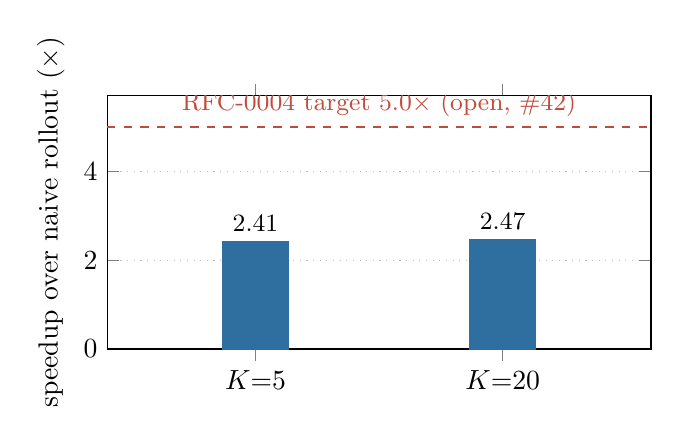
\begin{tikzpicture}
  \begin{axis}[
    width=0.7\linewidth, height=4.8cm, ybar, bar width=24pt,
    ymin=0, ymax=5.7,
    ylabel={speedup over naive rollout ($\times$)},
    symbolic x coords={$K{=}5$,$K{=}20$},
    xtick=data, enlarge x limits=0.6, ymajorgrids, grid style=dotted,
    nodes near coords, every node near coord/.append style={font=\small,/pgf/number format/.cd,fixed,precision=2},
  ]
  \addplot[fill=genocolor,draw=genocolor] coordinates {({$K{=}5$},2.41386) ({$K{=}20$},2.47322)};
  \draw[carboncolor,thick,dashed]
    ({rel axis cs:0,0}|-{axis cs:$K{=}5$,5.0}) -- ({rel axis cs:1,0}|-{axis cs:$K{=}20$,5.0})
    node[pos=0.5,above,font=\small,carboncolor]{RFC-0004 target $5.0\times$ (open, \#42)};
  \end{axis}
  \end{tikzpicture}
  \caption{\textbf{Historical KV-cache micro-benchmark.} Cached \texttt{ARPredictor} rollout is
  $2.41\times$ ($K{=}5$) and $2.47\times$ ($K{=}20$) faster than naive repeated one-step prediction.
  The gain is real but short of the $5\times$ target at $K{=}20$, which remains open and was explicitly rescoped.
  Measured on synthetic tensors with batch $8$, $d_{\mathrm{state}}{=}1024$, $d_{\mathrm{action}}{=}64$, CUDA, and bf16 on H200. The benchmark-specific predictor ($d_{\mathrm{hidden}}{=}1024$, $6+1$ blocks, FFN $4096$) is not the exact released checkpoint.}
  \label{fig:arspeed}
\end{figure}}

% ----------------------------------------------------------------------
% Figure: efficiency three-regime latency decomposition
% ----------------------------------------------------------------------
\newcommand{\figEfficiency}{%
\begin{figure}[t]
  \centering
  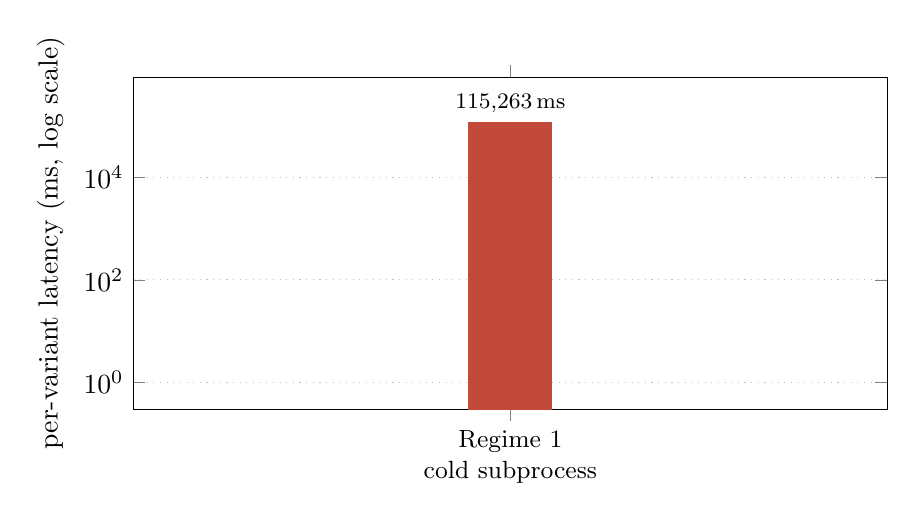
\begin{tikzpicture}
  \begin{semilogyaxis}[
    width=0.92\linewidth, height=5.8cm, ybar, bar width=30pt,
    ymin=0.3, ymax=900000, ymode=log, log origin=infty,
    ylabel={per-variant latency (ms, log scale)},
    symbolic x coords={Regime 1\\cold subprocess,Regime 2\\warm cache,Regime 3\\latent rollout},
    xtick=data, xticklabel style={align=center,font=\small},
    enlarge x limits=0.28, ymajorgrids, grid style=dotted,
    point meta=explicit symbolic,
    nodes near coords, every node near coord/.append style={font=\footnotesize,anchor=south},
  ]
  \addplot[fill=carboncolor,draw=carboncolor] coordinates {
    ({Regime 1\\cold subprocess},115262.94) [115{,}263\,ms]};
  \end{semilogyaxis}
  \end{tikzpicture}
  \caption{\textbf{Historical cold-process timing.} Only \emph{Regime 1}, a cold \texttt{geno-lewm-score} subprocess (interpreter start,
  ${\sim}1$\,GiB Carbon load, two Carbon forward passes), is measured, at $115{,}262.94$\,ms. The
  release did not profile component timing, so this total cannot be apportioned between loading and compute. The
  ``pay-Carbon-once'' thesis applies to \emph{Regime 2} (warm reference cache: one Carbon call on the
  edited window, in-process) and \emph{Regime 3} (latent-only rollout/planning: zero further Carbon
  calls), both \emph{unmeasured} on this checkpoint and therefore shown without bars. Because corresponding model quality is invalidated, this figure
  supports neither a deployment claim nor an efficiency--quality comparison.}
  \label{fig:efficiency}
\end{figure}}

% ======================================================================
% tables.tex  --  all result tables for the GenoLeWM paper.
% Every value is from the published v0.2.1-r1 readiness report / README.
% Carbon columns are recovered as (GenoLeWM value) - (reported delta).
% ======================================================================

% ----------------------------------------------------------------------
% Table 1: variant-effect prediction vs Carbon zero-shot
% ----------------------------------------------------------------------
\newcommand{\tabVEP}{%
\begin{table}[t]
  \centering
  \caption{\textbf{Variant-effect prediction (v0.2.1-r1).} Binary ClinVar slices report
  accuracy / AUROC / average precision (AP) / balanced accuracy; BRCA2 saturation and TraitGym
  Mendelian report Spearman $\rho$ against continuous functional/causal labels. The baseline is the
  same frozen Carbon-500M encoder scored zero-shot. $\Delta$ is GenoLeWM~$-$~Carbon (positive favours
  GenoLeWM). Bold marks the better value per row. GenoLeWM shows a positive delta only on coding-ClinVar
  accuracy/balanced accuracy ($+0.0625{=}1/16$, within quantization) and a TraitGym tie near zero; it
  trails on every pathogenicity-bearing ranking metric.}
  \label{tab:vep}
  \small
  \begin{tabular}{llrrr}
    \toprule
    Benchmark & Metric & GenoLeWM & Carbon 0-shot & $\Delta$ \\
    \midrule
    \multirow{4}{*}{ClinVar coding}
      & Accuracy \up           & \textbf{0.7500} & 0.6875 & $+0.0625$ \\
      & AUROC \up              & 0.7344 & \textbf{0.9219} & $-0.1875$ \\
      & AP \up                 & 0.8530 & \textbf{0.9519} & $-0.0989$ \\
      & Balanced acc.\ \up     & \textbf{0.7500} & 0.6875 & $+0.0625$ \\
    \midrule
    \multirow{4}{*}{ClinVar non-coding}
      & Accuracy \up           & 0.4375 & \textbf{0.6875} & $-0.2500$ \\
      & AUROC \up              & 0.5625 & \textbf{0.8750} & $-0.3125$ \\
      & AP \up                 & 0.6055 & \textbf{0.9144} & $-0.3090$ \\
      & Balanced acc.\ \up     & 0.4375 & \textbf{0.6875} & $-0.2500$ \\
    \midrule
    BRCA2 saturation   & Spearman $\rho$ \up & 0.1492 & \textbf{0.4769} & $-0.3277$ \\
    TraitGym Mendelian & Spearman $\rho$ \up & \textbf{$-0.0280$} & $-0.0839$ & $+0.0559$ \\
    \bottomrule
  \end{tabular}
\end{table}}

% ----------------------------------------------------------------------
% Table 2: latent rollout fidelity vs source-state baseline
% ----------------------------------------------------------------------
\newcommand{\tabRollout}{%
\begin{table}[t]
  \centering
  \caption{\textbf{Latent rollout fidelity (v0.2.1-r1).} Mean cosine similarity (\up) and mean $L_2$
  distance (\dn) between the predicted final state $\shat$ and the true encoded state $\stp$, over
  two multi-edit settings. The baseline predicts no change ($\shat{=}\st$). The do-nothing baseline
  dominates on both fidelity metrics, and Recall@4 is saturated at $1.0$ for \emph{both} the model and
  the baseline, so it does not discriminate. This is the latent-residual baseline trap
  (\cref{fig:rollout}).}
  \label{tab:rollout}
  \small
  \begin{tabular}{lrrrrrr}
    \toprule
    & \multicolumn{3}{c}{Cosine to $\stp$ \up} & \multicolumn{3}{c}{$L_2$ to $\stp$ \dn} \\
    \cmidrule(lr){2-4}\cmidrule(lr){5-7}
    Setting & GenoLeWM & Source-state & $\Delta$ & GenoLeWM & Source-state & $\Delta$ \\
    \midrule
    Phased haplotypes      & 0.2889 & \textbf{0.9978} & $-0.7090$ & 33.32 & \textbf{2.13} & $+31.19$ \\
    Synthetic edit chains  & 0.3016 & \textbf{0.9912} & $-0.6896$ & 28.80 & \textbf{3.17} & $+25.64$ \\
    \bottomrule
  \end{tabular}
\end{table}}

% ----------------------------------------------------------------------
% Table 3: inference efficiency + AR rollout speed
% ----------------------------------------------------------------------
\newcommand{\tabEfficiency}{%
\begin{table}[t]
  \centering
  \caption{\textbf{Measured efficiency (v0.2.1-r1, single NVIDIA H200).} The released
  single-variant score path is dominated by two frozen Carbon-500M forward passes under a cold cache
  and process start, so per-variant latency is $\approx$115\,s --- the architectural amortization thesis
  (\cref{fig:architecture}) is \emph{not} exercised by this naive path (\S\ref{sec:efficiency}). The
  KV-cached autoregressive rollout speedup is the only place latent-only cheapness appears, and it
  remains below the $5\times$ target at $K{=}20$.}
  \label{tab:efficiency}
  \small
  \begin{tabular}{lr}
    \toprule
    Quantity & Value \\
    \midrule
    Single-variant latency (cold, 2 Carbon passes) & $115{,}262.94$ ms ($\approx$115\,s) \\
    Batched throughput                             & $0.3095$ variants/s \\
    Peak memory                                    & $1{,}966{,}149{,}632$ B ($\approx$1.83\,GiB) \\
    \midrule
    AR rollout speedup, $K{=}5$  & $2.41\times$ \;(local $2\times$ target met) \\
    AR rollout speedup, $K{=}20$ & $2.47\times$ \;(RFC-0004 $5\times$ target \emph{not} met, \#42 open) \\
    \bottomrule
  \end{tabular}
\end{table}}

% ----------------------------------------------------------------------
% Table 4: artifact identity / reproducibility commitments
% ----------------------------------------------------------------------
\newcommand{\tabArtifacts}{%
\begin{table}[t]
  \centering
  \caption{\textbf{Content-addressed artifact identity for the evaluated release.} Every reported
  number is bound to these identities through checksum receipts; the benchmark suite re-renders its
  report (and this manuscript's machine-generated companion) from the artifacts and rejects stale text
  or mutated evidence (\S\ref{sec:reproducibility}). All 28 suite outputs verified.}
  \label{tab:artifacts}
  \small
  \begin{tabular}{ll}
    \toprule
    Field & Value \\
    \midrule
    Model release    & \texttt{geno-lewm-v0.2.1-r1} \\
    Model id         & \texttt{sha256:cddb8f3b9671\ldots f5f3ed6af4} \\
    Dataset snapshot & \texttt{geno-lewm-data-v0.2.1-r1} \\
    Commit           & \texttt{d9b06815cf8e\ldots5aa4154d} \\
    Hardware         & NVIDIA H200 (Linux x86\_64, glibc 2.35) \\
    Suite outputs    & 28 / 28 verified (\texttt{release\_inputs}: pass) \\
    \bottomrule
  \end{tabular}
\end{table}}


\title{Registered but Not Anticipated:\\
The Edit-Response Geometry of a Frozen Genomic Foundation Model}

\author{%
  Abdelhamid Bakhta\\
  \url{https://github.com/AbdelStark/GenoLeWM}
}

\begin{document}
\maketitle

\begin{abstract}
Latent world models promise to predict the consequence of an action in representation space,
skipping the encoder forward pass that would otherwise be needed to observe it. We ask whether
that promise holds for the most economical genomic action---a single-base edit---on frozen DNA
foundation-model features, and we find that it does not, for a reason that is
information-theoretic rather than architectural. We measure the \emph{edit-response geometry}:
the displacement $\Delta = s(\walt) - s(\wref)$ a point edit induces in a pooled state, over
$12{,}993$ GRCh38-grounded ClinVar and BRCA2 saturation-editing variants, across a pooling grid,
on three encoders that share neither objective nor tokenizer. Three findings follow. First, the
\emph{predict-no-change trap} is universal: a single edit leaves $\cos(s(\wref),s(\walt)) \ge
0.993$ on every encoder and every pooling width, reaching $1.00000$ under global pooling, so an
identity map wins any cosine-supervised objective---yet on \carbon{} the pathogenicity AUROC of
$\lVert\Delta\rVert$ stays flat at $0.92$--$0.93$ while the relative displacement varies
$9.4\times$. Dilution is not information loss; the trap is the metric, not the geometry. Second,
whether that geometry is \emph{informative} is an encoder-specific property, not a property of
genomic FMs: the same measurement gives AUROC $0.93$ on \carbon{}, $0.76$ on
Nucleotide~Transformer~v2, and $0.55$---near chance---on HyenaDNA. On \carbon{} the response is
interventional, exceeding a reference-only probe that never sees the edit by $0.13$--$0.31$ and
surviving conditioning on the full trinucleotide context ($-0.006$); on Nucleotide~Transformer~v2
at the same span it does not, the unedited window predicting better than the edit response.
Third, and independent of the first two, the pathogenicity-bearing component of the response is
precisely the component that cannot be anticipated: predicting $\Delta$ from the pooled reference
state and the action reaches AUROC $0.652$ against a $0.926$ ceiling, barely above the $0.631$
obtainable from the substitution class with no model at all, and the pooled state is not merely
uninformative but harmful (ridge $0.585$, below a lookup that ignores it). The failure deepens as
the state is pooled more, as an information-bottleneck account predicts. On \carbon{} the
geometry is not a restatement of the model's own likelihood: it beats $\Delta\log$-likelihood on
identical variants ($0.9255$ vs.\ $0.8945$), correlates with it only weakly ($\rho = -0.24$),
retains $0.853$ once it is residualised out, and ensembles to $0.948$. We report these AUROCs as
cohort-dependent---$\Delta\log$-likelihood reaches $0.89$ on our ClinVar slice against
$0.6$--$0.8$ in the literature, so the slice is easy---and we make no claim to a competitive
variant-effect predictor; transfer to quantitative function is weak ($\rho = -0.27$). These
results supersede our withdrawn \texttt{v0.2.1-r1} release, whose implementation defects were
real but incidental: the bottleneck we identify would have defeated a correct implementation too.
For an action-conditioned latent world model over pooled genomic features, there is no shortcut
through the latent---the encoder must be run on the edited sequence.
\end{abstract}

% ======================================================================
\section{Introduction}
\label{sec:intro}

DNA foundation models~\citep{dnabert2021,hyenadna2023,nucleotidetransformer2025,caduceus2024,evo2024}
answer a representational question: \emph{what is the embedding, or the likelihood, of this
sequence?} A different question is \emph{interventional}: given a reference genomic window and an
explicit edit, what is the \emph{consequence} of that edit in representation space? If a frozen
encoder's response to an edit could be \emph{anticipated}---computed from the reference state plus
a description of the edit, without re-running the encoder---then a static genomic encoder would
become an action-conditioned \emph{world model}~\citep{worldmodels2018,dreamerv3} whose actions are
discrete genomic edits, and whose latent transitions are cheap enough to score variants, roll out
haplotypes, and plan edit sets. That is the promise: one expensive encoder pass per reference
window, then arbitrarily many cheap latent queries (\cref{fig:architecture}).

This paper measures whether that promise can be kept, and reports that it cannot---for a reason more
general than any implementation. Our object of study is the \emph{edit-response geometry} of a
frozen DNA foundation model, principally \carbon~\citep{carbon500m}: the displacement
$\D=\salt-\sref$ induced in a pooled representation by a single-nucleotide edit. We measure it on
$14{,}000$ GRCh38-grounded variants across four pooling widths, and we ask three questions of it in
sequence. Does the frozen encoder \emph{register} the edit informatively? Is that a property of
genomic foundation models, or of Carbon? And can the registration be \emph{predicted} from the
pooled reference state and the action?

The answers dissociate, and the dissociation is the result. \emph{On Carbon}, the edit is registered
richly: $\D$ separates ClinVar pathogenic from benign SNVs at AUROC $0.9259$, and this survives
every control we could construct---restriction to SNVs, restriction to within a substitution class,
conditioning on the full trinucleotide context, and probes that see the reference locus but never
the edit. That richness, however, is \emph{Carbon's} and not the field's: run through two encoders
sharing neither objective nor tokenizer, the identical measurement on the identical variants gives
$0.7574$ on Nucleotide~Transformer~v2 and $0.5460$---near chance---on HyenaDNA
(\cref{sec:generality}). And on Carbon, where the response is worth predicting at all, it cannot be
anticipated. The best learned predictor of $\D$ from $(\sref,a)$ recovers AUROC $0.6520$, against a
ceiling of $0.9259$ from reading the encoder's true response, and against $0.6306$ available from
the substitution class alone with no model at all. Adding the pooled reference state to the action
buys approximately nothing---and under a linear model it is worse than nothing, scoring $0.5854$
against $0.6079$ for a lookup table that ignores the reference state entirely. \textbf{The
information exists; it is not where a latent world model needs it to be. There is no shortcut
through the pooled latent: you must run the encoder on the edited sequence.}

\paragraph{The predict-no-change trap, which \emph{is} universal.} A second measurement explains why
this failure mode is easy to misread, and why we consider the negative result worth reporting rather
than quietly abandoning. At global pooling, $\cos(\sref,\salt)=0.99989$: the edited state is
cosine-indistinguishable from the reference to four decimal places. Yet AUROC over those same states
is $0.9313$. An objective that asks a model to predict $\salt$ from $\sref$---which is what the
natural JEPA-style formulation asks---is therefore \emph{degenerate}: ``predict no change'' attains
the target to within $10^{-4}$ while carrying none of the discriminative signal. Dilution of the
edit under pooling is real and strong ($9.4\times$ in relative displacement), but it is \emph{not}
information loss. The trap is the metric, not the representation. An experiment that reports a
cosine gap under this formulation has measured its own objective, not the encoder. Unlike the
informativeness result, this one \emph{does} generalise: across all three encoders and every pooling
width, $\cos(\sref,\salt)\ge0.993$, reaching $1.00000$ for HyenaDNA at global pooling
(\cref{sec:generality}). It is a property of pooling a genomic FM, not of Carbon.

\paragraph{This is a measurement paper with a negative headline.} We did not build a working
genomic world model, and we do not claim one. We report what a frozen encoder's pooled edit
response contains, what it costs to obtain, and what cannot be learned from it. The intended
audience is other groups considering the same architecture; the intended saving is their compute.
We are also not proposing a variant-effect predictor: \cref{sec:scope} shows the measurement is
strong on curated binary labels and \emph{weak} on quantitative function (Spearman $-0.265$ on
BRCA2 saturation genome editing), and we report that as a limitation rather than an aside.

\paragraph{Contributions.}
\begin{enumerate}[leftmargin=1.4em,itemsep=1pt,topsep=2pt]
\item \textbf{An edit-response spectroscopy of \carbon} (\cref{sec:spectroscopy}): the
displacement induced by a single-base edit, measured across pooling widths on $14{,}000$
GRCh38-grounded variants, with the sensitivity ceiling ($\cos=0.99989$ at global pooling) and the
dissociation between that ceiling and a flat $0.92$--$0.93$ AUROC.
\item \textbf{A controlled demonstration that \carbon's response is interventional}
(\cref{sec:controls}): the signal is not the mutation spectrum ($0.6306$ with no geometry), not the
exact local sequence context (conditioning on the full trinucleotide context costs $0.0059$ AUROC),
and not the genomic neighbourhood ($0.6392$ from a reference-only probe, tracked by a
chromosome-held-out probe at $0.6354$, so not locus leakage).
\item \textbf{A propagation measurement} (\cref{sec:propagation}): the local and distal components
of the response point in genuinely different directions ($\cos=0.4714$), so pooling does not merely
rescale a local token swap; Carbon propagates the edit.
\item \textbf{A three-encoder generality test that splits the claim in two} (\cref{sec:generality}):
the same $12{,}993$ SNVs through Carbon, Nucleotide~Transformer~v2, and HyenaDNA show that the
predict-no-change trap is \emph{universal} ($\cos\ge0.993$ everywhere), while informativeness is
\emph{not} ($0.93 \to 0.76 \to 0.55$) and the interventional property is Carbon-specific---on
Nucleotide~Transformer~v2 at $\pm48$\,bp the unedited window predicts pathogenicity better than the
edit response does. This is why we scope the interventional claim to Carbon throughout.
\item \textbf{The core negative result} (\cref{sec:predict}): the pathogenicity-bearing component of
the edit response is precisely the component that is \emph{not} predictable from the pooled
reference state plus the action, with the failure worsening as the state is pooled more---as an
information-bottleneck account predicts.
\item \textbf{An explained retraction} (\cref{sec:retraction}): our own withdrawn
\texttt{v0.2.1-r1} release had real implementation defects, but we show the deeper reason it could
not have worked, and that a correct implementation would have failed too.
\end{enumerate}

\paragraph{What we do \emph{not} claim.} No clinical, diagnostic, or decision-support claim of any
kind. No claim that this is a competitive variant-effect predictor---and, as \cref{sec:loglik}
shows, our ClinVar slice is an easy one, so the AUROCs here are cohort-dependent and are not
comparable to published benchmark numbers. No claim about token-level world models, which we did not
test. No claim that Carbon's informative, interventional edit response generalises to genomic
foundation models at large: \cref{sec:generality} shows it does not, which is why every
interventional statement in this paper is scoped to Carbon by name. No claim about encoders larger
than $500$M or with longer contexts than we tested, and in particular no claim to know whether the
spread we measure tracks architecture, objective, or capacity. We collect these boundaries in
\cref{sec:limitations}.

\figArchitecture

% ======================================================================
\section{Related Work}
\label{sec:related}

\paragraph{Latent world models over frozen features.}
The template we test is DINO-WM~\citep{dinowm2025}, which learns an action-conditioned latent
forward model on top of frozen DINOv2~\citep{dinov2_2024} patch features and plans in latent space
by predicting future patch embeddings. \citet{sobal2025rewardfree} isolate what a latent dynamics
model buys over model-free alternatives on reward-free offline data; the Dreamer
line~\citep{dreamerv3} and TD-MPC2~\citep{tdmpc2_2024} establish, respectively, generative and
decoder-free latent dynamics for control, while PETS~\citep{pets2018} shows probabilistic dynamics
models suffice for control in a handful of trials; Ha and Schmidhuber~\citep{worldmodels2018} originate the
frozen-encoder plus latent-controller decomposition. Our setting differs in a way that turns out to
be decisive. These are \emph{high action-authority} domains: an action moves the state
substantially, so ``predict-no-change'' is a weak baseline and the target signal is rich. A
single-nucleotide edit moves a pooled genomic state by $\cos=0.99989$ at global pooling, so
predict-no-change is nearly unbeatable in absolute-state space, and the science has to move into
displacement space (\cref{sec:spectroscopy}). We are not planning; we are measuring the ceiling
that any such world model would be built against.

\paragraph{JEPAs and anti-collapse regularization.}
I-JEPA~\citep{jepa2023} predicts target-block representations from a context block without a pixel
decoder, and V-JEPA~2~\citep{vjepa2_2025} adds an action-conditioned variant enabling planning from
image goals---the closest visual analogue of the predictor we test, with an SNV as the action.
LeJEPA~\citep{lejepa2025}, by Balestriero and LeCun, proves that among embedding distributions at a
fixed covariance budget the isotropic Gaussian uniquely minimizes downstream probe bias, and
enforces it with \emph{SIGReg}: random one-dimensional projections with characteristic-function
matching, in linear time and memory. \textbf{We adopt LeJEPA's isotropic-Gaussian \emph{rationale},
not its estimator.} The regularizer in our own withdrawn release (\cref{sec:retraction}) was a
closed-form Gaussian KL to an isotropic target---a different and weaker mechanism than SIGReg,
which we describe here only so that run is characterized accurately. VICReg, Barlow Twins, and DINO
supply the surrounding anti-collapse toolbox. The difference from all of these is one of regime
rather than method: in vision, the masked target is high-uncertainty and information-rich; here the
target is $\approx99.99\%$ recoverable by copying the input, and the entire signal lives in the
residual.

\paragraph{Genomic foundation models and their variant-effect paradigm.}
Carbon is autoregressive and decoder-only with a $6$\,bp tokenizer, so, like Evo and
Evo~2~\citep{evo2024,evo2_2025}, GPN~\citep{gpn2023}, and HyenaDNA~\citep{hyenadna2023}, it
supports zero-shot $\Delta\log$-likelihood scoring; masked models such as the Nucleotide
Transformer~\citep{nucleotidetransformer2025}, DNABERT~\citep{dnabert2021}, and
Caduceus~\citep{caduceus2024} support pseudo-likelihood analogues. AlphaGenome~\citep{alphagenome2025}
and supervised track predictors are a contrast class: they score variants by comparing predicted
assay tracks, not by a likelihood or a state displacement. Carbon itself has no archival
publication; we cite the technical report and pin a model revision (\cref{tab:artifacts}). Every
one of these papers reports downstream VEP \emph{accuracy}; none characterizes the intrinsic
displacement geometry of a single edit, which is our object. We measure that geometry on three of
these models---Carbon, Nucleotide~Transformer~v2, and HyenaDNA---and one of our findings is that it
differs sharply between them (\cref{sec:generality}).

\paragraph{Variant-effect prediction: the $\Delta\log$-likelihood and embedding-distance paradigms.}
ESM-1v~\citep{esm1v2021} established that a frozen LM's log-likelihood ratio predicts mutation
effect with no task supervision, and GPN~\citep{gpn2023} and Evo~\citep{evo2024} carry the identical
idea into DNA; AlphaMissense~\citep{alphamissense2023} gives broader field context. Our nearest
methodological neighbour is \textbf{embedding-distance VEP}: BEND~\citep{bend2024} and general
in-silico-mutagenesis practice already use the distance between reference and alternate embeddings
as a variant score. That is precisely the quantity whose geometry we dissect. Prior work
\emph{thresholds} $\lVert\D\rVert$ as a black-box score; we characterize why it behaves as it does
and---the part that is new---ask whether it can be \emph{anticipated} rather than measured. The
evaluation resources are ClinVar~\citep{clinvar2014}, gnomAD~\citep{gnomad2020},
TraitGym~\citep{traitgym2025}, and MaveDB~\citep{mavedb2025}, specifically the BRCA2 saturation
genome-editing assay of \citet{sahu2025}.

\paragraph{The gap, and the closest concurrent work.}
Across this literature we find no systematic characterization of the pooled-state displacement
geometry of a single-nucleotide edit, and no test of whether that displacement is recoverable by an
action-conditioned latent predictor. The most direct concurrent neighbour is
JEPA-DNA~\citep{jepadna2026}, which grounds genomic FMs by predicting masked-segment latent
representations and improves linear-probe accuracy. It is a \emph{pretraining objective evaluated by
downstream accuracy}; ours is a \emph{measurement of single-edit displacement geometry and its
predictability}. The two are complementary, and---if our bottleneck account is right---JEPA-DNA's
choice to predict \emph{segment} rather than pooled representations is on the more promising side
of exactly the boundary we draw in \cref{sec:limitations}.

% ======================================================================
\section{Method}
\label{sec:method}

\subsection{Frozen encoder and the representation contract}
The encoder is \carbon~\citep{carbon500m}, a $500$M-parameter decoder-only DNA language model
(LLaMA-style, hidden size $1024$, $6$\,bp tokenizer), loaded at pinned revision \texttt{5d31d59b}
in \texttt{bf16} and \textbf{frozen throughout}. No encoder parameter is trained anywhere in this
paper. Each variant is placed at the centre of a $4{,}096$\,bp GRCh38 window. We take layer-$20$
hidden states $H\in\Real^{T\times 1024}$ and pool them to a state $s\in\Real^{1024}$.

Three contracts fix the measurement. We state them explicitly because the failure documented in
\cref{sec:retraction} was caused by leaving them implicit.
\begin{description}[leftmargin=1.2em,itemsep=1pt,topsep=2pt]
\item[Window.] Reference and edited windows are the same $4{,}096$\,bp interval, differing in
exactly one base for an SNV. The variant is at the window centre by construction.
\item[Pooling.] $s^{(r)}=\mathrm{mean}\big(H[c-r:c+r+1]\big)$ for radius $r\in\{8,64,256\}$ tokens,
where $c$ is the token index of the edited base, derived from the observed DNA-content offset after
Carbon's leading control token. Because the tokenizer is $6$\,bp, these radii are $\pm48$, $\pm384$,
and $\pm1536$\,bp. We write $r{=}0$ for global-mean pooling over the entire window, which is
therefore the \emph{widest} setting, not the narrowest: throughout, the pooling grid is ordered
$r{=}8 < r{=}64 < r{=}256 < \text{global}$ by width. Reference and edited states are always pooled
at the same centre with the same radius.
\item[Normalization.] All geometry is defined on raw pooled states. We report only quantities that
are explicitly scale-aware ($\lVert\D\rVert_2$) or explicitly scale-free ($\cos$,
$\lVert\D\rVert_2/\lVert\sref\rVert_2$), so that no comparison depends on an unstated normalization
convention.
\end{description}

\subsection{Definitions}
For a variant $v$ with reference window $\wref$ and edited window $\walt=\mathrm{apply}(v,\wref)$,
at pooling width $r$:
\begin{equation}
\label{eq:defs}
\sref=\enc(\wref),\qquad
\salt=\enc(\walt),\qquad
\D \;=\; \salt-\sref,
\end{equation}
and we report the \emph{relative displacement} and the \emph{state cosine}
\begin{equation}
\label{eq:geom}
\mathrm{rel}\D \;=\; \frac{\lVert\D\rVert_2}{\lVert\sref\rVert_2},
\qquad
\cos(\sref,\salt)\;=\;\frac{\langle\sref,\salt\rangle}{\lVert\sref\rVert_2\,\lVert\salt\rVert_2}.
\end{equation}
$\mathrm{rel}\D$ measures how far the edit moves the state relative to the state's own scale;
$\cos(\sref,\salt)$ measures how far it moves it in the metric a JEPA-style objective would
actually optimize. \Cref{sec:spectroscopy} shows these two tell the same story, and that both are
misleading about information content.

\subsection{Cohort}
The cohort is $14{,}000$ real GRCh38-grounded variants $\times\ 4$ pool radii $=56{,}000$ rows, with
$0$ skips: ClinVar~\citep{clinvar2014} $1{,}572$ pathogenic / $6{,}428$ benign, and $6{,}000$ BRCA2
saturation genome-editing variants~\citep{sahu2025} from MaveDB score set
\texttt{urn:mavedb:00001242-a-1}~\citep{mavedb2025}. Because the initial ClinVar set was not
SNV-only, and because indels displace the state far more than substitutions in a way that is aligned
with the label, all headline analyses restrict to SNVs: $12{,}993$ SNVs, of which ClinVar
contributes $899$ pathogenic and $6{,}094$ benign, with $1{,}007$ non-SNV rows excluded and counted.
Every one of the $12{,}993$ SNVs was checked against the reference FASTA and matched its recorded
reference base ($12{,}993/12{,}993$).

\subsection{Two further encoders, and the units that make them comparable}
\label{sec:encoders}

Everything above describes one encoder, and a measurement on one encoder cannot distinguish a
property of pooled genomic FM states from a property of Carbon. To separate them
(\cref{sec:generality}) we repeat the identical measurement on two further frozen encoders, chosen
to share as little as possible with Carbon or with each other:
\begin{description}[leftmargin=1.2em,itemsep=1pt,topsep=2pt]
\item[Nucleotide Transformer v2, $100$M multi-species~\citep{nucleotidetransformer2025}:] a
\emph{masked} language model---a different training objective---with a $6$\,bp tokenizer and
$d{=}512$.
\item[HyenaDNA-450k~\citep{hyenadna2023}:] implicit long convolutions rather than attention, and a
\emph{single-nucleotide} (character) tokenizer, with $d{=}256$.
\end{description}
Three objectives, two tokenizations, three widths. Both additional encoders are frozen at load, both
see the same $12{,}993$ SNVs in the same $4{,}096$\,bp windows at the same four pooling widths---%
$51{,}972$ rows each, $0$ skips---and both are processed by
\texttt{tools/research/edit\_response\_analysis.py} \emph{unchanged}, so no cross-encoder difference
we report can come from the analysis.

\paragraph{Radii are tokens; every comparison is in base pairs.} The pool radius $r$ is counted in
\emph{tokens}. Carbon and NT-v2 pack $6$\,bp into a token; HyenaDNA packs $1$. Comparing the three
at equal $r$ would therefore compare a $\pm48$\,bp pool against an $\pm8$\,bp one and call the
difference an encoder effect. We instead run HyenaDNA at radii $0,48,384,1536$ so that its pooling
windows match the others' $0,8,64,256$ at $0$ (global), $\pm48$, $\pm384$ and $\pm1536$\,bp, and we
label every cross-encoder axis, row, and column \textbf{in base pairs}. The distinction is not
cosmetic: a single base perturbs $1$ of $4{,}097$ character tokens against $1$ of $683$ $6$\,bp
tokens, which is the mechanism behind the encoder differences in \cref{tab:enctrap}.

\paragraph{A tokenizer hazard worth recording: NT-v2 re-anchors its grid on \texttt{N}.} NT-v2's
tokenizer packs $6$-mers greedily behind a leading \texttt{<cls>}, which makes the obvious mapping
from a genomic offset to a token index---$\lfloor \text{locus}/6\rfloor + 1$---look safe. It is not.
A $6$-mer containing an \texttt{N} is out of vocabulary; the tokenizer degrades to single-nucleotide
tokens across it and \emph{re-anchors the $6$-mer grid after it}. Any window containing an
\texttt{N}---and reference windows do---therefore has a token layout that the arithmetic mapping
silently gets wrong, and the pool is centred on the wrong tokens with no error raised anywhere. Our
tool instead reconstructs each token's span from the token strings themselves, verifies that the
reconstructed spans tile the window exactly, and fails closed on any \texttt{<unk>}. We record this
because the failure is silent and label-independent: it is precisely the class of defect that
survives review, and it is a close cousin of the pooling-coordinate defect that withdrew our own
earlier release (\cref{sec:retraction}).

\subsection{Predictability protocol and its baselines}
\label{sec:predict-protocol}
The world-model question, correctly posed, is not ``predict $\salt$ from $\sref$''---%
\cref{sec:spectroscopy} shows that target is $\approx99.99\%$ attained by copying the input. It is:
\emph{predict the displacement $\D$ from the reference state and the action, without encoding the
edited window.} That is exactly the efficiency thesis, and it is falsifiable.

The action space is the $12$ substitution classes (ordered base-to-base pairs); position is not an
action variable because every variant sits at the window centre by construction. We fit predictors
$\gpred(\sref,a)\to\Dhat$ under $5$-fold cross-validation on the $12{,}993$ SNVs, at radius
$8$---the most favourable, most local pooling width, chosen deliberately so that a failure there is
informative about every wider setting. We evaluate two things, and keeping them separate is
essential:
\begin{description}[leftmargin=1.2em,itemsep=1pt,topsep=2pt]
\item[Direction:] $\cos(\Dhat,\D)$, the fidelity of the predicted displacement direction.
\item[Magnitude:] AUROC of $\lVert\Dhat\rVert_2$ for ClinVar pathogenic vs.\ benign---whether the
predicted response carries the pathogenicity signal that the \emph{true} response carries.
\end{description}

\paragraph{The baseline ladder.} A negative result is only as good as what it is negative against,
so we bracket the learned predictors from below and above. From below: a \emph{global-mean $\D$}
predictor that ignores its inputs entirely; a \emph{per-substitution-class-mean lookup}, which is a
$12$-entry table with no learning; and \emph{the substitution class alone}, scored directly with no
displacement at all. From above: the \emph{TRUE $\D$} ceiling---what you get by paying for the
encoder pass. A world model is worth building only if it lands meaningfully above the lookup table
and near the ceiling.

\paragraph{Three method notes that constrain interpretation.}
First, \textbf{a cosine-trained predictor's magnitude is meaningless}: the cosine objective is
scale-invariant, so $\lVert\Dhat\rVert$ is unconstrained, and any AUROC computed from it is an
artifact of initialization and optimizer path rather than a measurement. We therefore report
AUROC$(\lVert\Dhat\rVert)$ \emph{only} for the MSE-trained predictor, and report the cosine-trained
predictor's direction only.

Second, the ridge baseline's $\lambda$ was swept over $1$--$10^{6}$ (best $10^{3}$) before we
concluded anything: an under-regularised failure would prove nothing. Ridge is fit with an
intercept. This detail is load-bearing rather than pedantic: an earlier prototype standardised a
design matrix containing a constant column, and because that column has zero standard deviation,
standardising annihilated it, leaving the model unable to represent $\mathbb{E}[\D]$. Every ridge
number reported here comes from the corrected fit.

Third, \textbf{AUROC is computed with averaged tied ranks}. This matters only for the model-free
baselines and it matters a great deal there: the global-mean predictor emits $5$ distinct
magnitudes and the class-mean lookup $60$, so ties dominate their score and a tie-naive
implementation misreports them. The MLP-MSE predictor emits $12{,}993$ distinct values with no
ties and is unaffected either way---which is why the headline is robust to this choice while the
baselines are not. All predictability numbers are those emitted by
\texttt{tools/research/delta\_predictability.py}, using the repository's tie-safe AUROC.

% ======================================================================
\section{Edit-Response Spectroscopy of \carbon}
\label{sec:spectroscopy}

This section measures \carbon\ alone; \cref{sec:generality} then asks which of its findings are
properties of Carbon and which are properties of pooling a genomic FM. The answer is not uniform, so
we name the encoder rather than the field throughout.

\subsection{The sensitivity ceiling: dilution is real, information loss is not}
\label{sec:ceiling}

\Cref{fig:sensitivity} sweeps the pooling width. Sensitivity peaks at the narrowest pool and decays
monotonically as the pool widens: mean $\mathrm{rel}\D$ is $0.0759$ at $r{=}8$, $0.0230$ at
$r{=}64$, $0.0101$ at $r{=}256$, and $0.0083$ at global pooling---a $9.4\times$ swing. The state
cosine mirrors it: $\cos(\sref,\salt)$ is $0.99352$ at $r{=}8$, $0.99925$ at $r{=}64$, $0.99984$ at
$r{=}256$, and $0.99989$ globally. Under global pooling a single-base edit is invisible to cosine at
four decimal places.

The natural inference is that pooling has destroyed the edit. It has not. Over the very same states,
ClinVar pathogenic-vs-benign AUROC is \emph{flat}: $0.9259$ at $r{=}8$, $0.9278$ at $r{=}64$,
$0.9313$ at $r{=}256$, and $0.9313$ globally (\cref{tab:controls}). The edit signal survives at
every pooling scale. What decays is not the information but its \emph{share of the norm}.

This dissociation is the paper's first substantive point, and it retro-diagnoses a whole class of
experiments including our own. \textbf{``Predict-no-change'' wins on cosine because cosine is the
wrong metric, not because the information is absent.} A predictor optimizing
$1-\cos(\hat s_{\mathrm{alt}},\salt)$ against a target that the identity function already reaches at
$0.99989$ is being scored almost entirely on a component of the problem that carries no signal. The
objective is degenerate by construction. Displacement space is not a stylistic preference here; it
is the only space in which the question is well posed.

Of everything in this section, this is the finding that generalises: \cref{sec:generality} shows the
same ceiling on a masked model and on a convolutional, character-level one, with
$\cos(\sref,\salt)\ge0.993$ at every encoder and every pooling width.

\figSensitivity

\subsection{\carbon's response is interventional, not a confound}
\label{sec:controls}

An AUROC of $0.93$ from a frozen encoder invites suspicion, so we tried to break it
(\cref{tab:controls}, \cref{fig:auroc}). Everything in this subsection is a statement about Carbon:
\cref{sec:generality} shows that the interventional conclusion we reach here is one Carbon earns and
the other two encoders we measured do not.

\paragraph{Not indels.} The raw cohort was not SNV-only, and indels displace the state far more than
substitutions in a way that correlates with the pathogenic label---an inflation aligned with the
outcome. Purging them ($1{,}007$ non-SNV rows, counted and excluded) leaves AUROC at $0.9259$ at
$r{=}8$. The signal was not the indels.

\paragraph{Not the mutation spectrum.} Some substitution classes are simply more often pathogenic,
and a model could exploit that without any geometry at all. Scoring by substitution class
alone---no displacement, no model---gives $0.6306$. Restricting the AUROC to comparisons
\emph{within} each of the $12$ substitution classes (covering $n{=}6{,}993$) leaves
$0.9202$--$0.9245$ across the sweep. The geometry carries far more than the spectrum, and it carries
it after the spectrum is held fixed.

\paragraph{Not the local sequence context either---the sharpest control.} The $12$-class control is
weaker than it looks, because it does not condition on local sequence, and a DNA language model's
response to a base swap plausibly depends on its immediate neighbours. So we ran the standard
mutational-signature decomposition (\cref{tab:trinuc}): condition on the full trinucleotide
context---the $5'$ base, the reference base, the $3'$ base---\emph{and} the substitution, then score
only within each context. This is the control a referee is most likely to demand, and it is the one
that could most plausibly have destroyed the result. It does not. Conditioning on the exact local
context costs $0.0059$ AUROC: $0.9305$ stratified against $0.9364$ unstratified, both measured on
the identical $5{,}027$ variants ($745$ pathogenic) covered by the $37$ contexts with at least $10$
variants per class. Meanwhile the trinucleotide lookup with zero geometry reaches
$0.6618$---above the $12$-class lookup's $0.6306$, as strictly more conditioning information should
be, and still far below the geometry. The edit response is not a restatement of mutation chemistry
or of local $k$-mer identity.

The apples-to-apples framing is load-bearing and we want to be explicit about it. The stratified
$0.9305$ exceeds the full-cohort unstratified $0.9259$ of \cref{tab:controls}, which would look like
stratification \emph{improving} the signal. It does not: the $37$ retained contexts cover a
different and slightly easier subset of the cohort, and against its own subset the stratified score
is a small \emph{decrease}. We report the comparison within the shared population because it is the
only one that licenses a conclusion.

We flag the limit of this control rather than let it be inferred: trinucleotide context spans
$\pm1$\,bp, whereas Carbon's tokenizer packs $6$\,bp into a token. It therefore does not fully
control for the exact ref-$6$-mer\,$\to$\,alt-$6$-mer token pair. The natural next stratification,
$\pm2$\,bp ($5$-mers), is too sparse to be powered at $899$ pathogenic variants, so we do not report
it (\cref{sec:limitations}).

\paragraph{Not the genomic neighbourhood.} This was the most serious threat: pathogenic variants
cluster in conserved, functionally dense regions, so a probe might recognise the \emph{locus} and
never need the edit. A linear probe on $\sref$ alone---which never observes the edit---reaches
$0.6392$ at $r{=}8$, and $0.5500$--$0.5741$ at the wider settings. To exclude locus leakage across
cross-validation folds, we re-ran the probe with chromosome-disjoint folds: $0.6354$ at $r{=}8$,
tracking the random-fold probe at every radius. There is no same-locus leakage, and the
neighbourhood explains at most $0.64$ of the $0.93$.

What remains, after the spectrum and the neighbourhood are removed and leakage is excluded, is the
edit itself. \carbon's response is \emph{interventional}. We are deliberate about the subject of
that sentence: run the same control on Nucleotide~Transformer~v2 at the same span and it inverts,
the reference-only probe beating the edit response ($0.7794$ against $0.7496$; \cref{sec:generality}).
The control is passed by an encoder, not by a field.

\figAUROC
\tabTrinuc

\subsection{Carbon propagates the edit}
\label{sec:propagation}

If a single-base edit merely rewrote its own $6$\,bp token, then the displacement at a wide pool
would be a scaled-down copy of the displacement at a narrow one, and the whole phenomenon would be
an uninteresting artifact of averaging. We test this directly by comparing displacement
\emph{directions} across pooling widths (\cref{fig:propagation}). Per variant,
$\cos(\D\text{ at global pooling},\ \D\text{ at }r{=}8)$ has mean $0.4714$, median $0.4721$, and
standard deviation $0.1905$; only a fraction $0.004$ of variants exceed $0.9$, and none exceed
$0.99$. A pure local token swap would put this distribution at $1.0$. It sits near $0.47$.

Magnitude \emph{ordering}, by contrast, is well preserved: Spearman between $\lVert\D\rVert$ at
global pooling and at $r{=}8$ is $0.8595$. The picture is coherent: \emph{which} variants move the
state a lot is stable across scales---which is why AUROC is flat---but \emph{where} they move it is
not. The distal response is a genuinely different direction from the local one. This is an
attention-mediated, context-dependent response, and the local and distal components independently
carry the signal. It also rules out the remaining deflationary reading of \cref{sec:ceiling}: the
flat AUROC under wide pooling is not a local vector surviving in miniature, it is a distinct global
response.

\figPropagation

% ======================================================================
\section{Generality: The Trap Is Universal, the Signal Is Not}
\label{sec:generality}

Everything in \cref{sec:spectroscopy} is a measurement of one encoder, and two quite different
claims are entangled in it. One is that a single edit barely moves a pooled genomic state, so any
absolute-state objective is degenerate---a claim about \emph{pooling}, which ought to hold for any
encoder. The other is that the displacement is informative and interventional---a claim we have so
far only licensed for \emph{Carbon}. A paper that leaves these fused generalises an $n{=}1$ result
by accident. So we ran the identical measurement, on the identical $12{,}993$ SNVs, through two
encoders that share neither training objective nor tokenizer with Carbon or with each other
(\cref{sec:encoders}), with the analysis code unchanged. The two claims come apart, and the second
one does not survive.

\subsection{The sensitivity ceiling replicates everywhere}

\Cref{tab:enctrap} reports the ceiling at bp-matched spans. It holds on all three encoders. The
lowest state cosine anywhere in the table is Carbon's $0.99352$ at $\pm48$\,bp, and since
$\pm48$\,bp is the \emph{maximum}-sensitivity span on all three, $\cos(\sref,\salt)\ge0.993$ at every
encoder and every pooling width. Under global pooling the edit is invisible to four decimal places
on Carbon ($0.99989$) and on NT-v2 ($0.99998$), and to five on HyenaDNA, whose cosine is
$1.00000$. The dilution curve has the same shape everywhere: sensitivity is highest at the narrowest
pool and falls as the pool widens ($\mathrm{rel}\D$ of $0.0759 \to 0.0083$ on Carbon,
$0.0889\to0.0050$ on NT-v2, $0.0130\to0.0008$ on HyenaDNA).

HyenaDNA is the extreme case, and the instructive one: its response is the smallest by roughly an
order of magnitude ($\mathrm{rel}\D = 0.0008$ globally against Carbon's $0.0083$; $0.0130$ against $0.0759$
at $\pm48$\,bp). Character tokenization predicts exactly this: a single base perturbs $1$ of
$4{,}097$ tokens rather than $1$ of $683$.

\textbf{This strengthens the paper's first claim rather than qualifying it.} The predict-no-change
trap is not an artifact of Carbon's tokenizer, its autoregressive objective, or its width. Across an
autoregressive model, a masked model, and a convolutional one, an objective that scores a predicted
edited state against the true one by cosine is being scored on a target the identity function
already attains to at least three decimal places. Anyone building an action-conditioned latent
predictor over pooled DNA-LM features will hit this, whichever encoder they pick.

\tabEncoderTrap

\subsection{Informativeness does not replicate, and the interventional property is Carbon's}

The second claim fails, and it fails in a graded way (\cref{tab:encoders}, \cref{fig:encoders}). The
same $\lVert\D\rVert$, on the same variants, from the same code, separates ClinVar pathogenic from
benign at $0.9313$ on Carbon, $0.7574$ on NT-v2, and $0.5460$---near chance---on HyenaDNA, under
global pooling; the ordering is stable across spans. Whether a frozen genomic FM's pooled state
registers a point edit \emph{usefully} is therefore not a property of genomic FMs. It is a property
of the encoder.

The sharper version concerns the control that \cref{sec:controls} rests on. The fair test of whether
the \emph{edit} beats the \emph{neighbourhood} is a supervised probe on $\D$ against the same
supervised probe on $\sref$, which never observes the edit; we write the difference $\D$~adds.
Carbon clears it at every span, by $+0.1346$ at $\pm48$\,bp, $+0.2967$ at $\pm1536$\,bp, and
$+0.3075$ globally. HyenaDNA adds $+0.0229$ to $+0.0303$---nothing, and from a base of chance.
NT-v2 adds $+0.1296$ and $+0.1326$ at the two wide spans but $\mathbf{-0.0298}$ at $\pm48$\,bp,
where its \emph{unedited} window ($0.7794$) predicts pathogenicity better than its edit response
does ($0.7496$). At that span, on that encoder, the interventional reading of \cref{sec:controls}
would be simply false: the probe is reading the locus, not the edit.

The three encoders are mechanistically consistent with one another. HyenaDNA's response at
$\pm48$\,bp is about $6\times$ smaller than Carbon's ($\mathrm{rel}\D$ $0.0130$ vs.\ $0.0759$) and
its AUROC is about chance. A weaker registered response carries a weaker signal, which is what one
would expect and is worth stating because it makes the spread legible rather than mysterious. The
BRCA2 transfer orders the same way, and is weak for both encoders that we measured on it: Spearman
$-0.265$ for Carbon against $-0.186$ for NT-v2.

\figEncoders
\tabEncoders

\subsection{What this licenses, and what it does not}

The claim we set out to make---\emph{frozen genomic FMs register point edits informatively}---is
false as stated, and \cref{tab:encoders} is what stopped us from publishing it. The claim we can
support is narrower and, we think, more useful:

\begin{quote}
Whether a frozen genomic FM's pooled state usefully registers a point edit is an
\textbf{encoder-specific} property. The predict-no-change trap, by contrast, is \textbf{universal}.
And even for the best of the three encoders, the response still cannot be anticipated from the
pooled state (\cref{sec:predict}).
\end{quote}

Two boundaries on this. First, we do not know \emph{what} the spread tracks. All three encoders are
at most $500$M parameters, and objective, tokenizer, width, context length, and training data all
vary together across them; a three-point comparison cannot attribute the $0.93$-to-$0.55$ range to
architecture rather than capacity, or to either rather than pretraining corpus. Second, and for the
same reason, nothing here predicts how a larger or longer-context model would behave. Carbon is the
existence proof that an informative interventional pooled edit response is \emph{possible}; it is
not evidence that it is typical. We take the honest reading to be that a group planning to build on
this geometry must measure it on their own encoder first, because the measurement is cheap and the
outcome is not predictable from architecture on the evidence we have.

% ======================================================================
\section{Predictability: The Core Negative Result}
\label{sec:predict}

Carbon registers the edit (\cref{sec:spectroscopy}), and of the three encoders we measured it is the
only one whose registration is worth anticipating at all (\cref{sec:generality}). A world model does
not need the encoder to register the edit; it needs to \emph{anticipate} that registration from the
reference state and the action, because anticipating it is the only thing that saves the encoder
pass. We now test that on Carbon---the best case available to us---under the protocol of
\cref{sec:predict-protocol}, at radius~$8$, the most favourable pooling width.

\Cref{tab:predict} and \cref{fig:predict} report the result. Reading the encoder's true response
gives AUROC $0.9259$. The best learned predictor of that response, an MLP on $(\sref,a)$ trained
with MSE, gives $0.6520$. The substitution class alone, with no model at all, gives $0.6306$. A
$12$-entry class-mean lookup table gives $0.6079$. A predictor that ignores its inputs entirely
gives $0.4939$, \ie chance, as it should.

The gap that matters is not the one between $0.6520$ and $0.9259$, though that gap is large. It is
the one between $0.6520$ and $0.6306$. \textbf{The entire contribution of the learned model---all of
it, including the pooled reference state, the nonlinearity, and the training---is the difference
between $0.6520$ and the $0.6306$ you get for free by looking up which base changed into which.}

\paragraph{Conditioning on $\sref$ is worse than useless.} The stronger statement is available from
the linear model, and it is worth stating precisely because it is counterintuitive. Ridge on
$(\sref,a)$ scores AUROC $0.5854$---\emph{below} the $0.6079$ of the class-mean lookup, which
ignores $\sref$ entirely and is a strictly less informed model. Direction agrees:
$\cos(\Dhat,\D)=0.1770$ for ridge against $0.2107$ for the action-only lookup. Giving a linear
predictor the pooled reference state does not merely fail to help; it degrades the prediction,
because $\sref$ contributes $1024$ dimensions of neighbourhood summary that are near-irrelevant to
the response and dilute the one signal (the substitution class) that is relevant. The nonlinear
cosine-trained MLP improves direction to $0.3228$, so some structure is recoverable, but the
MSE-trained model's magnitude---the component that actually carries the label---sits at $0.1949$
cosine and $0.6520$ AUROC. That the harness is faithful is confirmed by an exact identity: ridge on
the action alone reproduces the class-mean lookup to every digit ($\cos=0.2107$, AUROC $0.6079$),
as it must, since one-hot ridge is class means.

\paragraph{The radius trend confirms the mechanism.} If the cause is an information bottleneck in
the pooled state, then predictability should degrade as the state is pooled more, while the ceiling
stays flat. It does. At radius $8$ ($\pm48$\,bp, the most local state) the MLP-MSE predictor reaches
$0.6520$ against a ceiling of $0.9259$. At global pooling it collapses to $0.5400$---essentially
chance---with $\cos(\Dhat,\D)=0.0575$, against a ceiling that is, if anything, \emph{higher} at
$0.9313$. The ceiling is flat in the pooling width; the predictability is not. The wider the pool,
the less the response can be anticipated, even though the response stays equally informative. That
is precisely the signature of a bottleneck: the pooled state summarises the neighbourhood while
discarding the local sequence context---which $6$-mer token is being rewritten, and in what
immediate surround---that determines the response.

\paragraph{The conclusion, stated plainly.} The pathogenicity signal in the edit response is exactly
the part that is not predictable from the pooled reference state plus the action. A latent world
model over Carbon's pooled states cannot recover it---not because the predictor is too small or the
optimizer too weak, but because the conditioning information is not in $\sref$. The efficiency
thesis fails at its premise. And it fails in the most favourable case we could construct: Carbon is
the one encoder of the three whose edit response is informative enough to be worth anticipating
(\cref{sec:generality}), so it is the one with the most to lose here. We tested predictability only
on Carbon, and we do not extrapolate the negative to encoders we did not test---but an encoder whose
response is uninformative offers a world model less to predict, not more. \textbf{There is no
shortcut through the pooled latent: you must run the encoder on the edited sequence.}

\figPredict
\tabControls
\tabPredict

% ======================================================================
\section{Baselines and Scope}
\label{sec:scope}

\subsection{Quantitative function: where the measurement is weak}
\label{sec:brca2}

The $0.93$ AUROC is on curated binary labels, and we do not want it read as a variant-effect result.
\Cref{tab:scope} reports the harder test. On the BRCA2 saturation genome-editing assay of
\citet{sahu2025} ($n{=}6{,}000$, radius $8$), Spearman between $\lVert\D\rVert$ and the measured
functional score is $-0.265$ (permutation $p<0.001$). Transferring the direction learned on ClinVar
gives $\rho=-0.155$.

These correlations are statistically real and practically weak, and the contrast with $0.93$ is the
honest content of this section. Two things differ between the evaluations. ClinVar is
ascertainment-biased toward clear-cut variants---it is a curated record of what clinicians
confidently called, so its positives and negatives are drawn from the tails. BRCA2 sGE, by contrast,
spans all SNVs in one gene's exons at fixed context, including the entire ambiguous middle, and asks
for a graded quantity rather than a binary one. Separating curated extremes is a much easier problem
than ordering a functional gradient. \textbf{This is not a competitive variant-effect-prediction
method and must not be presented as one.} We report the BRCA2 number because it bounds what the
geometry measurement is good for.

\tabScope

\subsection{Relation to the model's own likelihood, and the difficulty of our cohort}
\label{sec:loglik}

An AUROC of $0.92$ from a frozen encoder's displacement geometry is \emph{higher} than the
$0.6$--$0.8$ typically reported for zero-shot $\Delta\log$-likelihood variant scoring with DNA
language models~\citep{gpn2023,evo2024,esm1v2021}. A referee should not accept that at face value,
and neither should we. There are two readings. Either our ClinVar slice is unusually easy, or
embedding displacement genuinely beats likelihood surprise on this task. The measurement that
discriminates between them is Carbon's own $\Delta\log$-likelihood scored on the \emph{same}
variants: it is the standard score behind those published numbers, so it doubles as a
\emph{difficulty calibration} of our cohort. We report it at radius $8$, joined to the geometry on
$(\text{chrom},\text{pos},\text{ref},\text{alt})$, on $n{=}6{,}981$ ClinVar SNVs ($893$ pathogenic),
in \cref{tab:scope}.

Both readings turn out to be partly right, and we state each plainly because they are easy to
mistake for a contradiction. They are not: the first is about our \emph{cohort}, the second about
our \emph{quantity}.

\paragraph{(a) Our cohort is easy, and every AUROC in this paper is cohort-dependent.}
$-\Delta\log$-likelihood reaches AUROC $0.8945$ on this slice. That is far above what the same score
attains in the published zero-shot DNA-LM literature, and it is a fact about our data rather than
our method. \textbf{Our ClinVar slice is easy, and that---not a superior score---is the reason our
raw AUROC exceeds the literature's.} ClinVar ascertainment is the obvious mechanism
(\cref{sec:limitations}): the record contains what clinicians confidently called, so its positives
and negatives are drawn from the tails. We therefore report $0.9255$ as a cohort-dependent
measurement and explicitly \emph{not} as an absolute win over likelihood scoring; nothing here
licenses a claim that this geometry is a better variant-effect predictor than
$\Delta\log$-likelihood on any cohort but ours, and the weak BRCA2 transfer (\cref{sec:brca2})
points the same way.

\paragraph{(b) But on identical variants the geometry carries orthogonal signal.} Calibration is not
the whole story, because the two scores are computed on the same $6{,}981$ variants and they do not
agree with each other. $\lVert\D\rVert$ scores $0.9255$ against the likelihood's $0.8945$. They are
only weakly correlated: Spearman$(\lVert\D\rVert,\Delta\log\mathrm{Lik}) = -0.2391$. Residualising
$\lVert\D\rVert$ on $\Delta\log$-likelihood in rank space---deleting everything the likelihood
explains---still leaves AUROC $0.8529$. And a rank ensemble of the two reaches $0.9482$, above
either alone, which is the signature of two partly independent measurements rather than one measured
twice. The pattern survives the trinucleotide stratification of \cref{sec:controls}: within context,
$\lVert\D\rVert$ scores $0.9302$ against the likelihood's $0.9007$ ($n{=}5{,}021$, $64$ contexts).
On BRCA2 the two separate further: Spearman with the functional score is $-0.2649$ for
$\lVert\D\rVert$ against $+0.1124$ for $\Delta\log$-likelihood. Both are weak---this is the section
that says so---but the likelihood carries almost nothing there.

The consequence is a scoping claim, not a performance claim. \textbf{$\lVert\D\rVert$ is not a
restatement of likelihood surprise.} A frozen encoder's pooled displacement and its next-token
distribution register overlapping but distinct things about the same edit, which is why the
embedding-distance paradigm~\citep{bend2024} is not simply a noisy proxy for the
$\Delta\log$-likelihood paradigm~\citep{esm1v2021,gpn2023,evo2024}, and why the geometry was worth
dissecting rather than replacing with a likelihood. It is also why \cref{sec:predict} is
ceiling-relative and untouched by any of this: whatever $\lVert\D\rVert$ measures, and however easy
the cohort, the part of it that carries the label is the part a world model cannot anticipate.

\paragraph{A numerical hazard we walked into, and that others will.} Our first attempt at this
measurement was invalid, and the failure mode is worth a paragraph because it is silent and the
quantity is a standard one. Computed in \texttt{bf16}---the precision at which every other
measurement in this paper runs---$90.7\%$ of the $\Delta\log$-likelihoods came back \emph{exactly}
zero, and the survivors took only $18$ distinct values, every one a multiple of $16$. Nothing was
wrong with the model, the data, or the code. A $4{,}096$\,bp window's log-likelihood has magnitude
$\approx5{,}000$, and the spacing between adjacent representable \texttt{bf16} values at that
magnitude \emph{is} $16$: a single-base edit changes the window log-likelihood by far less than one
unit in the last place, so the difference is annihilated before it can be formed. The reported run
is \texttt{fp32}, on which the same pipeline yields $0$ exact zeros, $9{,}115$ distinct values, and
a range of $-486.0$ to $+36.3$. \textbf{Do not accumulate or difference log-likelihoods in
\texttt{bf16}.} We cite no number from the \texttt{bf16} run anywhere in this paper. The general
lesson is cheap to apply: before interpreting any distribution of differences, count its exact zeros
and its distinct values---a large mass of exact zeros over a small set of evenly spaced levels is a
float artifact, not a finding.

% ======================================================================
\section{Why the Released Run Failed, and Why a Correct One Would Have Too}
\label{sec:retraction}

This project previously released \texttt{v0.2.1-r1}: an action-conditioned latent predictor over a
frozen Carbon encoder, trained to predict $\hat s_{t+1}$ from $(s_t,a)$, benchmarked on ClinVar,
BRCA2, and TraitGym, and published with content-addressed receipts binding every reported number to
its bytes. Its results were withdrawn. That combination is the cautionary part: reproducible
execution reproduces an invalid computation just as faithfully as a valid one, so provenance has to
be paired with tested scientific contracts rather than mistaken for them~\citep{reproducibility2021}.
This section preserves that record, and then makes the point that matters: the defects were real,
but they are not the reason the idea could not work.

\subsection{What was actually broken}

A post-release audit established four defects, each verified against the released artifacts
(\cref{tab:rollout}, \cref{tab:vep}).

\paragraph{The normalization contract was ignored.} The configuration set \texttt{normalize: true},
but the encoder returned raw pooled states while the predictor always returned a unit-norm vector.
On the released rollout slices, mean source/target norms were $33.982/33.595$ (phased) and
$29.253/29.089$ (synthetic), against a mean prediction norm of $1.000$. Every $L_2$ loss, surprise
score, and rollout distance therefore compared operands differing by a factor of $\approx30$, and
was dominated by scale rather than by content.

\paragraph{Pooling coordinates were mismatched.} Training encoded source states with no edit locus
supplied, which silently triggered global-mean fallback, while targets were pooled around the edit.
Source and target states were thus in different coordinate frames. Separately, every ``centered''
pool omitted Carbon's leading \texttt{<dna>} control token and was shifted one hidden token left,
sometimes centering the pool on the control token itself.

\paragraph{The regularizer had no gradient.} The run was labelled \texttt{phase2}, but the encoder
remained frozen with no LoRA parameters, and its Gaussian KL term was computed only from frozen
target states---constant with respect to every trainable parameter, contributing exactly zero
gradient. No Phase-2 claim was tested by it.

\paragraph{The runtime was not self-contained.} The pinned Carbon \texttt{tokenizer.py} performed an
unpinned, network-capable transitive load of \texttt{Qwen/Qwen3-4B-Base}, so hashing the local
tokenizer file did not define the tokenizer that actually ran.

Consequently the released $L_2$ losses, surprise scores, $L_2$ rollout metrics, and every conclusion
drawn from them do not evaluate the intended method. The released cosine values ($0.289$ and $0.302$
prediction-to-target, versus $0.998$ and $0.991$ source-to-target) remain reproducible historical
measurements---cosine is scale-invariant---but they are confounded by mixed-scale, mixed-pooling
training and by train/rollout distribution shift, and they establish neither capability nor
mechanism. The run used seed $271828$, $10{,}000$ optimizer steps, and $80{,}000$ samples; its
ClinVar slices were $N{=}16$. We preserve these numbers in \cref{tab:vep} and \cref{tab:rollout},
and their identity in \cref{tab:artifacts}, for auditability; we withdraw the interpretations.

\subsection{The lesson the defects do not teach}

That audit explains why \emph{that run} was uninterpretable. It is silent on whether the idea was
sound. It is tempting---and it was our first reading---to conclude that the engineering was at fault
and that a corrected rerun would settle the question. \Cref{sec:predict} says otherwise.

Consider a hypothetical corrected \texttt{v0.2.1}: normalization applied consistently, source and
target pooled at the same token-layout-derived centre, a gradient-bearing regularizer, a
self-contained tokenizer, matched train and rollout distributions, and adequately powered slices. It
would have failed anyway, for two compounding reasons that no amount of engineering removes.

\textbf{First, its objective was degenerate.} It trained $\gpred(s_t,a)\to\hat s_{t+1}$ against a
target with $\cos(s_t,s_{t+1})=0.99989$ at global pooling (\cref{sec:ceiling}). The identity
function attains that target to four decimal places. A corrected run would have converged to a
near-copy of its input and reported a good-looking loss, and the loss would have measured nothing,
because the discriminative content lives in a residual the metric barely weighs. Fixing the
normalization bug would have made the numbers \emph{coherent} without making them
\emph{informative}.

\textbf{Second, and fatally, the conditioning information was absent.} Even after moving to the
correctly-posed displacement objective---which is what \cref{sec:predict} does, with a clean
implementation on clean data---the best predictor of $\D$ from $(\sref,a)$ recovers $0.6520$ of the
$0.9259$ available, barely above the $0.6306$ that requires no model at all. The pooled state is an
information bottleneck that discards precisely the local sequence context determining the edit
response. This is a property of Carbon's pooled frozen features---the very features that release was
built on---and not of our optimizer, our architecture, or our bugs. It would have been true of a
bug-free implementation. It would have been true of a better-designed one.

This is why we consider the reframe honest rather than convenient. A retraction that says ``we had
bugs'' generalises to nobody. The measurement says something stronger and more useful: this
architecture---an action-conditioned latent world model over the pooled frozen states this release
was built on---cannot deliver its premise, and the reason is information-theoretic rather than
engineering. Two of its components generalise beyond Carbon and one does not, and we are careful
about which: the degenerate cosine objective is a trap on every encoder we measured
(\cref{sec:generality}), whereas the claim that there was a rich response to anticipate in the first
place is one only Carbon earns. That converts a local embarrassment into a result other groups can
act on, and it is the reading the data supports.

\tabVEP
\tabRollout

% ======================================================================
\section{Limitations}
\label{sec:limitations}

We state these as constraints on the claim, not as caveats to it. Several are severe.

\paragraph{The claim is about \emph{pooled} states only.} We show that the edit response cannot be
anticipated from a pooled reference state plus an action. Pooled states are what latent world models
actually use, which is why the result bites. But we have \emph{not} shown that a token-level world
model is impossible, and nothing here argues that it is. A predictor operating on the full
hidden-state sequence retains the local context that pooling discards, and is the natural follow-up.
Our result draws a boundary; it does not close the area behind it.

\paragraph{Three encoders, none larger than $500$M.} An earlier draft of this paper carried a
limitation headed ``one encoder'', conceding that a single-model result was an anecdote about Carbon
until replicated. \Cref{sec:generality} replaced that concession with a measurement, and the
measurement changed the claim rather than confirming it: the predict-no-change trap replicated on
all three encoders, and the informative, interventional edit response did not replicate on either of
the other two. What was a caveat is now a result, and the paper is scoped accordingly---Carbon by
name wherever the response is called interventional.

What remains untested is the direction the replication did \emph{not} go. All three encoders are at
most $500$M parameters and share our $4{,}096$\,bp window, so we cannot say whether a larger or
longer-context model behaves like Carbon or like HyenaDNA. Nor can a three-point comparison
attribute the $0.9313$-to-$0.5460$ spread to any single cause: objective, tokenizer, width, context
length, and pretraining corpus all covary across these models, so the spread may track capacity or
training objective rather than architecture as such. \textbf{We do not claim to know which}, and a
reader who wants an answer should measure their own encoder rather than interpolate ours. Carbon is
additionally held at one revision, one layer, and one window length; that much of the original
limitation stands.

\paragraph{The action space is $12$ substitution classes.} Because every variant sits at the window
centre by construction, position carries no information and the action reduces to which base changed
into which. A richer action space---position, local sequence context, the identity of the rewritten
$6$-mer---is not tested here. This cuts against us in a specific and important way: a predictor
given the local context we withheld might do better than $0.6520$. We regard this as the most
credible route to overturning our negative result, and it is the same route as the token-level
follow-up above.

\paragraph{The $6$-mer token pair is not fully controlled.} Our trinucleotide control
(\cref{tab:trinuc}) conditions on $\pm1$\,bp, but Carbon's tokenizer packs $6$\,bp into a token, so
the exact ref-$6$-mer\,$\to$\,alt-$6$-mer token-pair confound survives it. The natural fix, a
$\pm2$\,bp ($5$-mer) stratification, is too sparse to be powered at $899$ pathogenic variants, and
we do not report an underpowered version of it. The trinucleotide result therefore bounds the
$k$-mer explanation without eliminating it.

\paragraph{ClinVar ascertainment bias, and it is measured, not merely suspected.} ClinVar records
what was confidently classified, which biases it toward clear-cut variants at the tails of the
effect distribution. We can put a number on how much this flatters us: Carbon's own
$\Delta\log$-likelihood, the standard zero-shot DNA-LM variant score, reaches AUROC $0.8945$ on our
slice against the $0.6$--$0.8$ it attains in the published literature (\cref{sec:loglik}). \textbf{Our
slice is easy}, and that---not the merit of the geometry---is why our raw AUROCs exceed the
literature's. AUROC $0.9259$ should be read as separation of curated extremes on a favourable
cohort, not as accuracy on the variants that are clinically difficult, which are exactly the ones
anybody needs help with. Every AUROC in this paper is cohort-dependent and none of them are
comparable to a benchmark number.

\paragraph{BRCA2 is one gene.} The quantitative-function evaluation ($\rho=-0.265$) covers a single
gene's exons in a fixed context, from a single assay. It bounds the claim in the direction of
weakness, and it should not be extrapolated in either direction to other genes or assays.

\paragraph{Not a variant-effect method.} We report AUROC against controls to characterize a
representation, not to compete on a benchmark. We do not compare against tuned VEP methods, we do
not tune ours, and the BRCA2 result indicates it would not compete.

\paragraph{No clinical claim of any kind.} Nothing in this paper is a clinical, diagnostic, or
decision-support tool or claim. No pathogenicity label enters any encoder, and no output here should
inform any decision about any person.

% ======================================================================
\section{Conclusion}
\label{sec:conclusion}

We measured the edit-response geometry of frozen genomic foundation models and found a clean
dissociation. \carbon \emph{registers} a single-base edit richly: the pooled displacement separates
ClinVar pathogenic from benign SNVs at AUROC $0.9259$, and it does so interventionally---not via the
mutation spectrum ($0.6306$ with no geometry), not via the exact local sequence context
(conditioning on the full trinucleotide context costs $0.0059$), not via the genomic neighbourhood
($0.6392$ from a probe that never sees the edit, with no locus leakage), and not via a local token
swap (distal and local response directions agree at only $\cos=0.4714$). Carbon propagates the edit
through attention, and the signal survives at every pooling width, even where the edit is
cosine-invisible ($0.99989$). It is not a restatement of the model's own likelihood either: on
identical variants it beats $\Delta\log$-likelihood ($0.9255$ vs.\ $0.8945$), correlates with it at
only $\rho=-0.2391$, and survives residualising it out ($0.8529$). The AUROCs are cohort-dependent
and the cohort is easy---the likelihood's $0.8945$ says so---so none of this is a variant-effect
claim.

Two of those sentences have Carbon as their subject on purpose. Run through two encoders sharing
neither objective nor tokenizer, the same measurement on the same variants gives $0.7574$ and
$0.5460$, the latter near chance, and Nucleotide~Transformer~v2's edit response is beaten at
$\pm48$\,bp by a probe on its own unedited window. Whether a frozen genomic FM's pooled state
usefully registers a point edit is an \emph{encoder-specific} property. The predict-no-change trap
is not: $\cos(\sref,\salt)\ge0.993$ on all three encoders at every pooling width, reaching
$1.00000$. The trap is what generalises; the signal is what does not.

And on Carbon, where the response is worth anticipating, it cannot be \emph{anticipated}. The best
learned predictor of the response from the pooled reference state plus the action recovers AUROC
$0.6520$ of the $0.9259$ available, against $0.6306$ free from the substitution class alone. The
reference state buys almost nothing, and a linear model conditioned on it does worse ($0.5854$) than
a lookup table that ignores it ($0.6079$); predictability degrades toward chance as pooling widens
while the ceiling stays flat. The pathogenicity-bearing component of the edit response is exactly
the unpredictable one.

The consequence for the architecture we set out to build is unambiguous, and negative. An
action-conditioned latent world model over Carbon's pooled features cannot deliver its premise,
because the premise is that you can skip the encoder pass on the edited sequence, and the encoder
pass is where the signal is created---and Carbon is the most favourable of the three encoders we
measured. Our own withdrawn \texttt{v0.2.1-r1} run had genuine implementation defects, but the
defects were not the reason it failed; a correct implementation would have failed too, and now we
can say why. The information exists. It is not where a latent world model needs it to be.
\textbf{There is no shortcut through the pooled latent.}

\section*{Acknowledgments}
We thank the maintainers of the open genomic-modeling and self-supervised-learning ecosystems whose
models, benchmarks, and methods this study builds on. Portions of the evidence-gathering, citation
verification, and manuscript drafting were assisted by AI research tooling.

{\small
\bibliographystyle{plainnat}
\bibliography{refs}
}

\appendix
% ======================================================================
\section{Notation}
\label{app:notation}
\begin{center}\small
\begin{tabular}{ll}
\toprule
Symbol & Meaning \\
\midrule
$\wref,\walt$ & reference / edited DNA window ($4{,}096$\,bp, variant at centre) \\
$\enc(\cdot)$ & \carbon (rev.\ \texttt{5d31d59b}), layer $20$, mean pool at radius $r$, raw \\
$\sref,\salt$ & pooled reference / edited state, $\Real^{1024}$ \\
$\D=\salt-\sref$ & the edit response (displacement); the object of study \\
$\mathrm{rel}\D$ & $\lVert\D\rVert_2/\lVert\sref\rVert_2$, relative displacement \\
$r$ & pool radius \textbf{in tokens}; $6$\,bp per Carbon token, so $r{=}8,64,256 \equiv
\pm48,\pm384,\pm1536$\,bp. \\
& HyenaDNA is $1$\,bp per token and is run at $r{=}48,384,1536$ to match in bp
(\cref{sec:encoders}). \\
& All cross-encoder comparisons are reported in base pairs, never in $r$. \\
$r{=}0$ & global-mean pooling over the whole window (the \emph{widest} setting) \\
$a$ & the action: one of $12$ substitution classes \\
$\gpred(\sref,a)\to\Dhat$ & the predictor under test; the ``shortcut'' \\
$n$ & $14{,}000$ variants; $12{,}993$ after SNV restriction; $6{,}993$ ClinVar SNVs \\
\bottomrule
\end{tabular}
\end{center}

\section{Artifact Identity and Provenance}
\label{app:artifacts}
\tabArtifacts

\section{Citation Verification Notes}
\label{app:citations}
Bibliography metadata was checked against publisher pages, DOIs, or arXiv where available. The
following caveats apply and should be resolved before any camera-ready version.
\begin{itemize}[leftmargin=1.4em,itemsep=1pt,topsep=2pt]
\item \textbf{Carbon has no archival publication.} There is a Hugging Face model card and a
\texttt{tech-report.pdf} in \texttt{github.com/huggingface/carbon}; no arXiv or journal version
exists. We cite it as a technical report and pin model revision \texttt{5d31d59b}. A moving GitHub
artifact is a legitimate reviewer objection; the tech report should be archived.
\item \textbf{LeJEPA attribution and mechanism.} LeJEPA is by Balestriero and
LeCun~\citep{lejepa2025}, and its estimator is SIGReg (random one-dimensional projections with
characteristic-function matching). Our withdrawn release used a closed-form Gaussian KL inspired by
the isotropic-Gaussian rationale; it is \emph{not} SIGReg, and \cref{sec:related} states this.
\item \textbf{BRCA2 source disambiguation.} There are two distinct Nature-2025 BRCA2 saturation
genome-editing papers. We cite \citet{sahu2025}, DOI \texttt{10.1038/s41586-024-08349-1}, and
\emph{not} the separate study at DOI \texttt{10.1038/s41586-024-08388-8}.
\item \textbf{MaveDB accession.} The score set \texttt{urn:mavedb:00001242-a-1} is the identifier
recorded by our data pipeline for the BRCA2 sGE scores. Its mapping to \citet{sahu2025} should be
confirmed directly on mavedb.org before assertion.
\item \textbf{Author lists.} \citet{jepadna2026} is confirmed as arXiv:2602.17162
(February 2026) and its author list was retrieved from the arXiv API. \citet{vjepa2_2025},
\citet{dinov2_2024}, and \citet{mavedb2025} have truncated author lists.
\item \textbf{Unconfirmed venue.} \citet{dinowm2025} is confirmed as arXiv:2411.04983; its
ICLR-2025 acceptance is inferred from OpenReview and not confirmed.
\item \textbf{Unconfirmed DOIs.} The \citet{evo2_2025} and \citet{alphagenome2025} entries cite
bioRxiv DOIs, which are solid; their journal DOIs were not confirmed and are not cited.
\end{itemize}

\end{document}
